% Beschreibung der anvisierten Bedienoberfläche (z.B. durch einen Prototyp oder frei gezeichnet) und Erläuterung der Menüstruktur.

In diesem Kapitel werden die Anforderungen an die Benutzeroberfläche genannt und beschrieben. Außerdem wird ein möglicher Entwurf dargestellt, der die Anforderungen erfüllt. Gegliedert ist das Kapitel dabei in die Anforderungen, die in jedem Fall erfüllt werden müssen, und jene, die je nach Möglichkeit umgesetzt werden.

\section{Hauptfenster}

\begin{figure}[h]
	\centering
	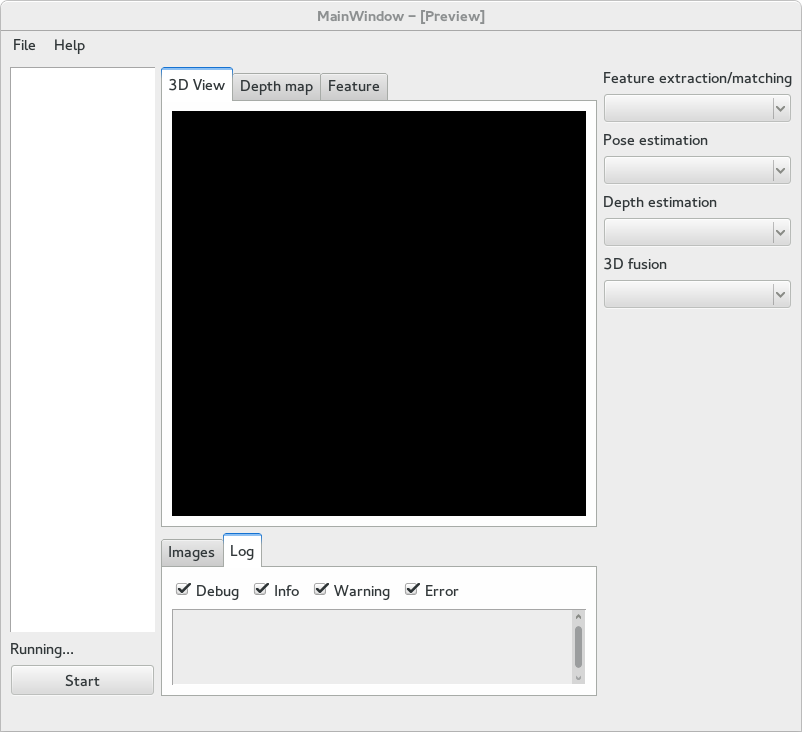
\includegraphics[width=0.9\textwidth]{img/Screenshot.png}
	\caption{Hauptfenster}
	\label{fig:Hauptfenster}
\end{figure}

\begin{enumerate}[ align=left, label={\textbf{\textbackslash B10\arabic*0\textbackslash}} ]
	\item \textbf{Algorithmenauswahl} Algorithmen können dem Workflow entsprechend aus ComboBoxen gewählt werden.
	\item \textbf{Bilderinput} Über den Eintrag „File → Load images...“ in der Menüleiste können Bilder als Eingabe der Algorithmen ausgewählt werden.
	\item \textbf{Bildervorschau} \label{B10Bildervorschau} Die Bilder, die als Eingabe für die Algorithmen gewählt worden sind, werden in einer Vorschau als Thumbnails angezeigt. In der Vorschau können einzelne oder mehrere Bilder ausgewählt werden, so dass sie in \ref{B10AnsichtsauswahlFeatures} dargestellt werden.
	\item \textbf{Starten} \label{B10Starten} Ein Button soll den Start der Ausführung der ausgewählten Algorithmen ermöglichen.
	\item \textbf{Arbeitsindikator} Pro Algorithmus wird dem Benutzer durch ein Symbol oder einen Text angezeigt, ob der Algorithmus gerade läuft.
	\item \textbf{Stoppen} Über ein Button kann der Nutzer die Ausführung der Algorithmen anhalten.
	\item \textbf{Ergebnisanzeige} Die Ergebnisse werden nach Möglichkeit zentral und groß dargestellt.
	\item \textbf{Ansichtsauswahl} Der Nutzer soll zwischen folgenden Ansichten wählen können:
		\begin{enumerate}[ label={\textbf{\alph*}}, ref={\textbf{\textbackslash B10\arabic{enumi}0\textbackslash\alph*}} ]
			\item 3D-Ansicht
			\item Tiefenkarte
			\item \label{B10AnsichtsauswahlFeatures} Features auf einem Bild, falls in \ref{B10Bildervorschau} ein Bild gewählt ist bzw. des Matchings von Features auf mehreren Bildern, falls mehrere Bilder gewählt sind
		\end{enumerate}
	\item \textbf{Protokoll} Dem Benutzer soll ein Protokoll über die Ausführung der Algorithmen bereit gestellt werden. Die verschiedenen Arten vom Protokollmeldungen (Fehler, Warnung, Info, Debug) sollen einzeln ein- und ausgeblendet werden können.
	\item \textbf{Speichern des Workflows} Die Algorithmenauswahl und der gewählte Workflows, falls vorhanden, sollen gespeichert werden können. Dafür stehen in der Menüleiste die Einträge „File → Save workflow“ und „File → Save worflow As...“ bereit.
	\item \textbf{Speichern der Ergebnisse} Die Ausgabedaten der Algorithmen können über die Einträge „File → Save results“ und „File → Save results As...“ in der Menüleiste gespeichert werden.
\end{enumerate}

\newpage

\section{Erweitertes Hauptfenster zur Umsetzung von Kann-Kriterien}

\begin{figure}[h]
	\centering
	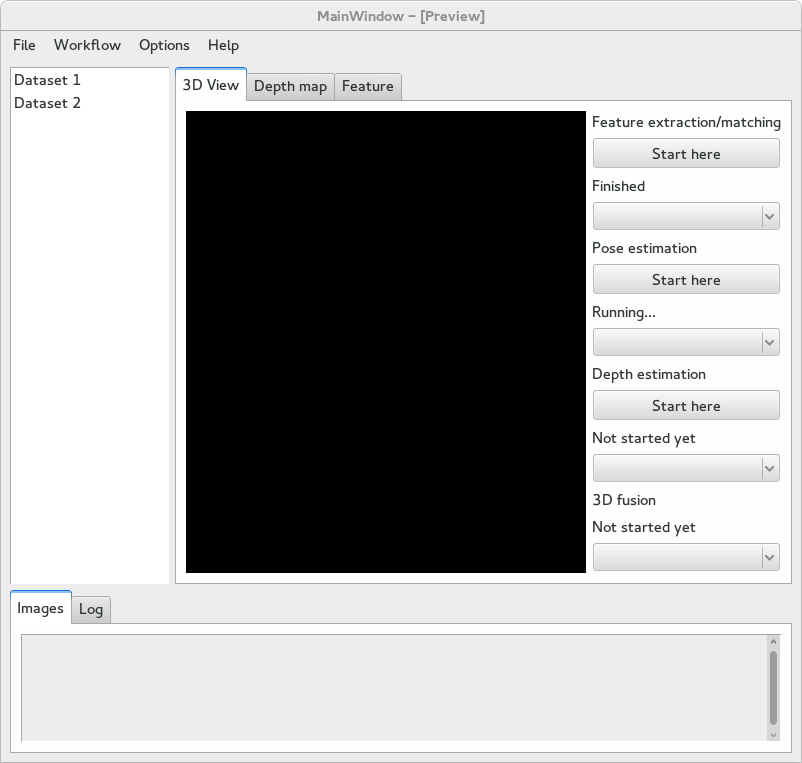
\includegraphics[width=0.9\textwidth]{img/Screenshot_advanced.png}
	\caption{Erweitertes Hauptfenster}
	\label{fig:Erweitertes Hauptfenster}
\end{figure}

Hinzugekommen ist:
\begin{enumerate}[ align=left, label={\textbf{\textbackslash B20\arabic*0\textbackslash}}]
	\item \textbf{Workflowauswahl} Dem Anwender wird eine Auswahl an Workflows in der Menüleiste unter dem Punkt „Workflow“ angeboten. Ein Workflow besteht aus verschiedenen Schritten, die festlegen, welche Algorithmen für einen Schritt ausgewählt werden kann.
	\item \textbf{Laden von Ausgabedaten der Algorithmen} \label{B20AlgorithmenDatenLaden} Über den Eintrag „File → Advanced load files...“ können die Ausgabedaten von vorherigen Läufen der Algorithmen geladen werden.
	\item \textbf{Starten ab einem bestimmten Algorithmus} Für jeden Algorithmus, der die Vorbedingungen erfüllt, gibt es einen Button, der es dem Nutzer ermöglicht diesen Algorithmus und alle nachfolgenden Algorithmen auszuführen. Vorbedingung heißt, dass dem Algorithmus alle Daten zur Ausführung vorliegen. Diese Daten stammen entweder aus vergangen Läufen der vorhergehenden Algorithmen in der gleichen Sitzung oder wurden vom Nutzer manuell durch \ref{B20AlgorithmenDatenLaden} geladen. Die Implementierung dieses Punktes ersetzt \ref{B10Starten}.
	\item \textbf{Auswahl der 3D-Darstellung} Mittels einer ComboBox kann der Nutzer die 3D-Darstellung zwischen folgenden Ansichten umschalten:
		\begin{enumerate}[ label={\textbf{\alph*}}, ref={\textbf{\textbackslash B20\arabic{enumi}0\textbackslash\alph*}} ]
			\item \textbf{Point cloud} zeigt die einzelnen Eckpunkte des 3D-Modells an.
			\item \textbf{Mesh} \label{B203DMesh} stellt die Oberfläche des 3D-Modells dar.
			\item \textbf{Textured} stellt das Mesh [\ref{B203DMesh}] inklusive der auf die Oberfläche gezeichneten Texturen da.
		\end{enumerate}
	\item \textbf{Mehrere Datensätze} Über eine Liste können mehrere Datensätze innerhalb einer Sitzung genutzt und verwaltet werden. Der Nutzer wird so in die Lage versetzt einen Workflow auf verschiedenen Eingabedaten zu evaluieren, ohne für jeden Test die Daten neu laden zu müssen.
\end{enumerate}